\chapter{Didaktické príklady}
\label{Didaktické príklady}

Pre AeroShield bolo v prostredí Arduino IDE, MATLAB a Simulink vytvorených niekoľko vzorových programov, ktoré demonštrujú všetky jeho funkcie. Programy sú rozdelené do dvoch veľkých skupín, konkrétne programy v otvorenej slučke bez spätnej väzby a programy v uzavretej slučke so spätnou väzbou. 

Ich rozdiel spočíva v tom, že pri riadení bez spätnej väzby, hovoríme o ovládaní systému, kedy sa snažíme dosiahnuť žiadané hodnoty výstupov bez spätnej informácie o vykonaní procesu, alebo o jeho hodnote. V prípade riadenia so spätnou väzbou sa jedná o reguláciu. Pri regulácii sa kontroluje bezprostredný účinok riadenia, ktorý sa porovnáva so žiadanou hodnotou výstupu a na vyrovnanie ich vzájomnej chyby, sa okamžite vykonáva zásah do vstupných veličín. 

\section{Programy v otvorenej slučke, bez spätnej väzby}
\subsection{Arduino IDE}
\label{bezspatnej}

Ako prvý príklad si ukážeme program s názvom \verb|AeroShield_OpenLoop.ino| napísaný v prostredí Arduino IDE. Hlavnou ideou tohoto programu je jednoduché ovládanie otáčok motorčeka pomocou potenciometra. Na začiatku programu inicializujeme hlavnú knižnicu AeroShieldu pomocou príkazu \verb|#include "AeroShield.h"|. Následne deklarujeme premenné, ktorých hodnoty budú vypisované na sériový monitor. 

\begin{lstlisting}[caption={AeroShield open loop dekleracia.},captionpos=b]
	float startangle=0;           //  Premenna pre nulovy uhol
	float lastangle=0;            //  Premenna pre maximalny uhol 
	float pendulumAngle;          //  Uhol natocenia kyvadla
	float referencePercent;       //  Hodnota potenciometra
	float CurrentMean;	      //  Hodnota prudu odoberaneho motorom 
\end{lstlisting}

V časti \verb|setup()| ako prvé prebehne nastavenie rýchlosti sériovej komunikácie \newline\verb|Serial.begin(115200)|. Číslo 115 200 predstavuje počet zmien, stavu z 0 na 1 resp. zo stavu high na stav low, za sekundu. Toto tempo signálnej rýchlosti nazývame \verb|baud rate|. Nasleduje funkcia \verb|AeroShield.begin()|, ktorá sleduje prítomnosť magnetu, a prednastaví potrebné premenné a funkcie pinov. Poslednou funkciou je kalibrácia kyvadla \verb|AeroShield.calibration()|, spolu s výpočtom začiatočného a koncového uhla kyvadla. 

\begin{lstlisting}[caption={AeroShield open loop setup().},captionpos=b]
	void setup() {                // Setup prebehne len jeden krat 
		Serial.begin(115200);       // Zaciatok seriovej komunikacie 
		AeroShield.begin();  // Inicializacia AeroShieldu 
		startangle = AeroShield.calibration(AeroShield.getRawAngle());   // Kalibracia kyvadla
		lastangle=startangle+1024;  // Kalkulacia uhlu kyvadla pre map function
	}
\end{lstlisting}

V cykle \verb|loop()| prebehne ako prvé mapovanie uhlu kyvadla pomocou funkcie \newline\verb|AutomationShield.mapFloat()|. Nasleduje čítanie hodnoty potenciometra, ktorá slúži na ovládanie akčného člena pomocou funkcie \verb|AeroShield.actuatorWrite()|. Na sériový súradnicový zapisovač sa modrou farbou vykreslí uhol kyvadla, červenou farbou hodnota potenciometra a zelenou veľkosť prúdu odoberaného motorom Obr. \ref{OBRAZOK 3.1}. 

\begin{lstlisting}[caption={AeroShield open loop loop().},captionpos=b]
	void loop() {
		referencePercent= AeroShield.referenceRead();  // Citanie potenciometra
		AeroShield.actuatorWrite(referencePercent); // Pohyb akcneho clenu
		CurrentMean= AeroShield.currentMeasure();  // Meranie prudu
		
		Serial.print(pendulumAngle);    
		Serial.print(" ");
		Serial.print(referencePercent);  
		Serial.print(" ");
		Serial.print(CurrentMean);   
		Serial.println(" ");
	}
\end{lstlisting}

\begin{figure}[!tbh]
	\centering
	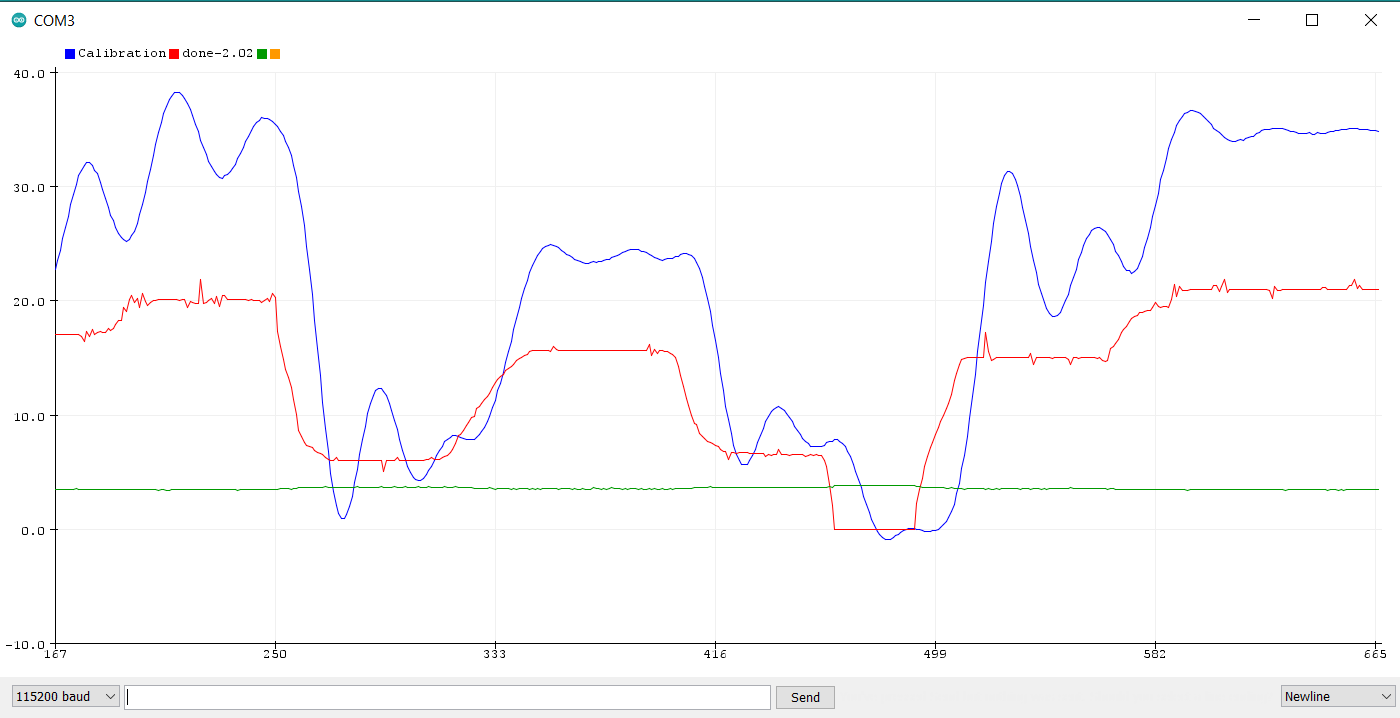
\includegraphics[width=120mm]{obr/VystupOLIDE.png}
	\caption{Výstup z programu AeroShieldOpenLoop.ino.}\label{OBRAZOK 3.1}
\end{figure}

\newpage
\subsection{MATLAB}
\label{MatlabPID}

V príklade \verb|AeroShieldOpenLoop.m| si ukážeme výhody a možnosti zobrazovania výstupov, v prostredí MATLAB. 

Na začiatku kódu vymažeme všetky premenné a objekty pomocou série príkazov \code{Clear all, clc}. Následne načítame knižnicu AeroShieldu a vykonáme funkciu \verb|AeroShield.begin()|. Kód pokračuje kalibráciou nulového uhlu kyvadla, zadefinovaním premenných na počítanie času, ako aj premenných na ukladanie hodnôt potenciometra a uhlu kyvadla. 

\begin{lstlisting}[caption={AeroShield open loop inicializacia.},captionpos=b]
	% vymazanie premennych a objektov 
	clear all
	clc 
	
	% nacitanie kniznice AeroShieldu  
	AeroShield=AeroShield;
	% vytvorenie objektov arduino, as5600
	AeroShield.begin();
	% kalibracia
	startangle= AeroShield.calibration(); 
	lastangle=startangle+2048; 
	
	% premenne na pocitanie casu
	time = 0;
	count = 0;
	angle = 0;          % uhol kyvadla
	potentiometer = 0;  % hodnota potenciometra
\end{lstlisting}

Nasleduje while cyklus, ktorý je ukončený zatvorením vykresľovaného grafu. V cykle najskôr čítame hodnotu potenciometra pomocou príkazu \verb|AeroShield.referenceRead()| a túto hodnotu zapisujeme na akčný člen príkazom \verb|AeroShield.actuatorWrite()|. Pokračujeme čítaním uhlu kyvadla \verb|AeroShield.getRawAngle()|, za ktorým prebehne mapovanie premennej z hodnoty raw na stupne. Premenná \verb|count| slúži na počítanie počtu prejdených cyklov, na tvorbu usporiadaného radu premenných, ako aj na vykresľovanie pohyblivej x-ovej osi grafu Obr. \ref{OBRAZOK 3.2}. Ľavá stupnica grafu je stacionárna a zobrazuje hodnotu potenciometra, pravá stupnica zobrazuje uhol kyvadla v stupňoch a svoje rozpätie zväčšuje, alebo zmenšuje v závislosti na výchylke kyvadla. Na konci programu ešte nájdeme if podmienku, ktorá kontroluje uhol kyvadla, ktorý ak nadobudne hodnotu väčšiu ako 110°, proces automaticky ukončí a vypíše upozornenie. Posledný príkaz \verb|clear AeroShield.arduino| vymaže objekt \verb|arduino| a pripraví MATLAB na spustenie ďalšieho programu. 

\begin{lstlisting}[caption={AeroShield open loop, while cyklus.},captionpos=b]
	while ishandle(plotGraph)           % slucka bezi pokial sa nezatvori graf
	
	pwm = AeroShield.referenceRead();   % citanie hodnoty potenciometra
	AeroShield.actuatorWrite(pwm);      % zapis na aktuator
	RAW= AeroShield.getRawAngle();      % citanie raw uhlu
	angle_ = mapped(RAW, startangle, lastangle, 0, 180); % mapovanie raw uhol na stupne
	
	count = count + 1;                              % zaznamenavanie poctu cyklov
	time(count) = toc;                              % zaznamenavanie casu
	angle(count) = angle_(1);                       % hodnota uholu v case 
	percenta= mapped(pwm, 0.0, 5.0, 0.0, 100.0);    % mapovanie pwm na percenta
	potentiometer(count) = percenta(1);             % hodnota potenciometra v case
	set(plotGraph,'XData',time,'YData',angle);      % vykresli prve data
	set(plotGraph1,'XData',time,'YData',potentiometer); % vykresli druhe data  
	axis([time(count)-5 time(count) 0 100]);        % beziaca x-ova osa
	
	if (angle_ > 110)                            % ak uhol kyvadla vacsi ako 110 stupnov 
	AeroShield.actuatorWrite(0.0);      % zastav motor  
	disp('Angle of pendulum too high. AeroShield is turned off')
	break                               % zastav program
	end
	end  
	
	clear AeroShield.arduino;           
\end{lstlisting}

\begin{figure}[!tbh]
	\centering
	\includegraphics[width=\textwidth]{obr/ASOLmat.png}
	\caption{Výstup z programu AeroShieldOpenLoop.m.}\label{OBRAZOK 3.2}
\end{figure}

\subsection{Simulink}


Na ukážku funkcií jednotlivých blokov \verb|AeroLibrary|, bol v API Simulink zostavený inštruktážny príklad \verb|AeroShieldOpenLoop| Obr. \ref{OBRAZOK 2.6.111}. V tomto príklade sa pomocou hodnoty potenciometra ovláda akčný člen. Zároveň je meraný uhol, v ktorom sa kyvadlo nachádza a obe tieto hodnoty sú priebežne zobrazované na grafe pomocou bloku \verb|Scope| Obr. \ref{OBRAZOK 3.22}. 

\begin{figure}[!tbh]
	\centering
	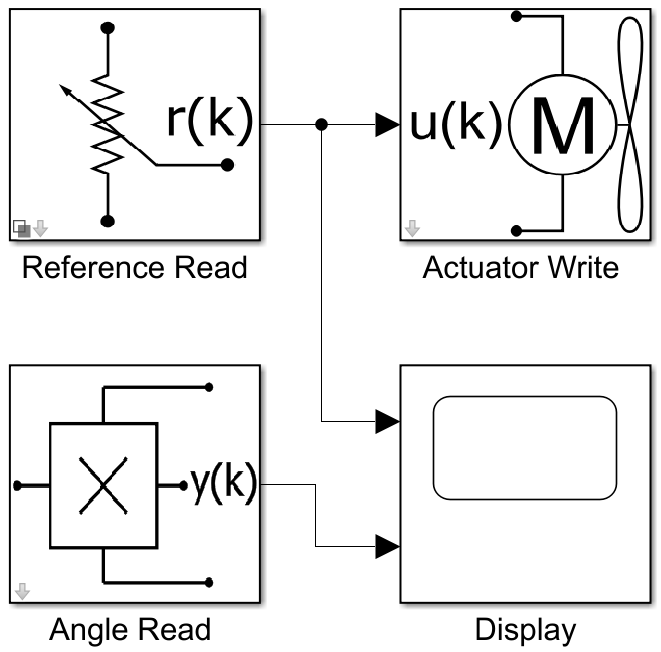
\includegraphics[width=90mm]{obr/AeroOpenLoop.png}
	\caption{AeroShield\_OpenLoop.}\label{OBRAZOK 2.6.111}
\end{figure}

\begin{figure}[!tbh]
	\centering
	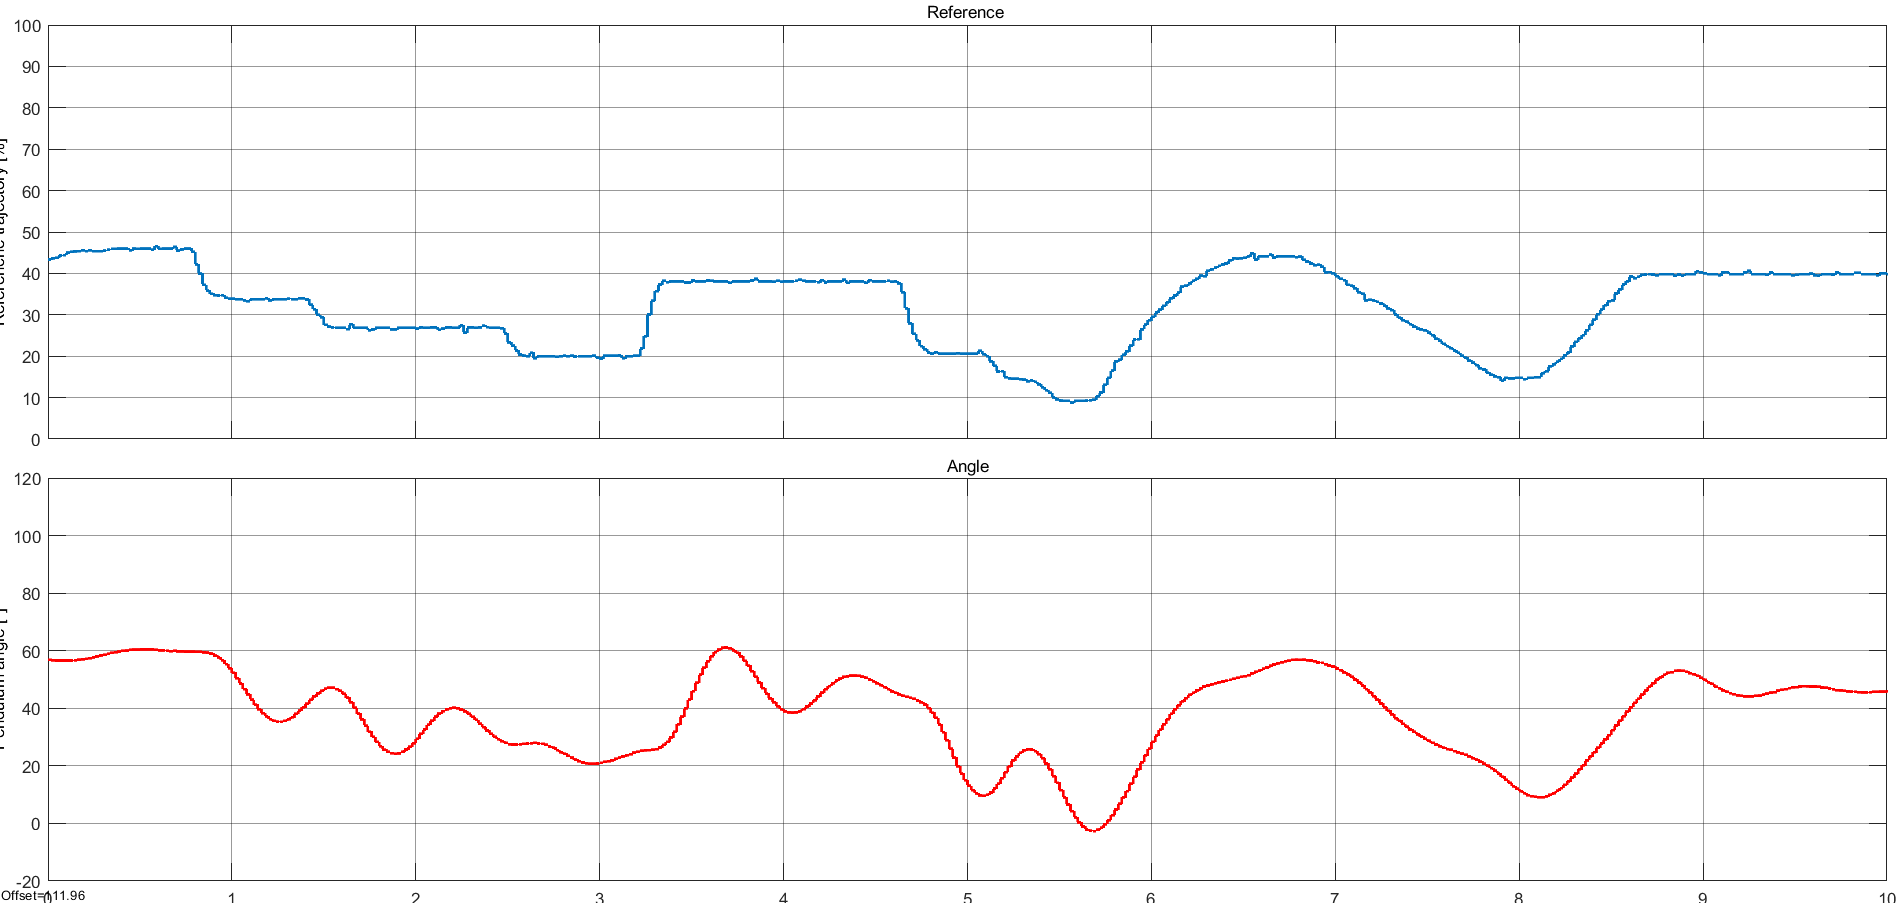
\includegraphics[width=120mm]{obr/SSmulinkOpenloop.png}
	\caption{Výstup z programu AeroShieldOpenLoop.sim.}\label{OBRAZOK 3.22}
\end{figure}



\chapter{PID regulácia}
\label{PIDPID}

PID reguláciu sme si vybrali z dôvodu jednoduchosti použitia, ako aj z dôvodu že práve PID regulácia je vyučovaná medzi prvými v rámci teórie riadenia. P, PI alebo PID regulátory taktiež patria medzi veľmi populárne typy riadiacich algoritmov.  

Skôr ako si ukážeme príklady s využitím PID regulátora, musíme si vysvetliť ako takýto regulátor funguje. Základom je získavanie informácii o sledovanej resp. riadenej veličine, za pomoci senzoru a jej porovnávanie s hodnotou žiadanou. Vďaka tomu, že získavame informácie o výstupe, ktoré aktívne využívame na riadenie akčného člena, môžeme hovoriť o spätnoväzbovom riadení. Spätnoväzbové riadenie, je teda také riadenie, ktoré ovplyvnuje sústavu na základe aktuálne získaných informácii o stave, v ktorom sa sústava nachádza. Pri takomto riadení existuje množstvo algoritmov, ktoré ovládajú správanie sa systému. Medzi tieto algoritmy patrí napríklad: Lineárne riadenie s premenlivým parametrom (LPV), Lineárno-kvadratické riadenie (LQ), Modelové prediktívne riadenie (MPC), Proporcionálno-integračno-derivačné riadenie (PID)...

PID regulátor Obr. \ref{OBRAZOK 3.3}, ovplyvňuje akčné zásahy do sústavy \verb|u(t)| na základe zaznamenaných výstupných informácii \verb|y(t)|. Veľkosť akčného zásahu \verb|u(t)| vypočítame na základe rozdielu medzi požadovanou hodnotou \verb|w(t)| a hodnotou reálnou \verb|y(t)|. Tento rozdiel označujeme tiež ako regulačná odchýlka \verb|e(t)|. Písmeno ,,t'' v zátvorkách predstavuje, časovú závislosť premenných. 

\begin{figure}[!tbh]
	\centering
	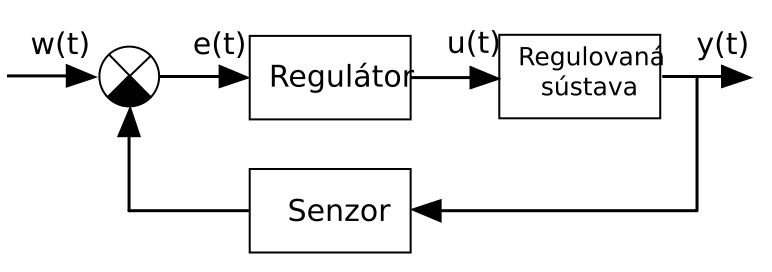
\includegraphics[width=120mm]{obr/pid.png}
	\caption{Schéma riadenia PID regulátorom.}\label{OBRAZOK 3.3}
\end{figure}

Skratka PID je zložená zo začiatočných písmen zložiek, z ktorých sa regulátor skladá. 

\begin{itemize}
	\item \textbf{P}- označuje tzv. proporcionálnu zložku. Akčný zásah \verb|u(t)|, je priamo úmerný veľkosti regulačnej odchýlky \verb|e(t)|. K$_p$ predstavuje proporcionálnu konštantu, ktorou násobíme regulačnú odchýlku na získanie požadovaného vstupu Rov. \ref{rovnicajedna}. 
	\begin{align}
		\label{rovnicajedna}
		u(t)=K_p e(t)
	\end{align}
	Konštanta K$_p$ je veľmi dôležitou pri nastavovaní parametrov PID regulátora. Zvyšovaním hodnoty proporcionálnej zložky znižujeme regulačnú odchýlku, avšak nikdy nedosiahneme úplne odstránenie trvalej regulačnej odchýlky. Zmenou proporcionálnej zložky vieme taktiež urýchliť, alebo spomaliť nábeh na požadovanú hodnotu. Pre malé hodnoty K$_p$ je nábeh pomalý, a regulačná odchýlka veľká. Pri zvyšovaní hodnoty K$_p$ sa zrýchľuje nábeh, no zároveň narastá nežiadúce kmitanie sústavy. Zvyšovanie hodnoty K$_p$ má svoj limit, za ktorým sa sústava dostáva za hranicu stability a ďalšia regulácia nie je možná. 
	
	\item \textbf{I}- predstavuje integračnú zložku. Integrálny riadiaci člen je priamo úmerný veľkosti chyby, ako aj dobe jej trvania. Pokiaľ má regulovaná veličina menšiu hodnotu ako je požadovaná, integrálna časť PID sa zväčšuje. Naopak pokiaľ je hodnota regulovanej veličiny väčšia ako požadovaná, integrálna časť PID klesá. Pri použití integračnej zložky PID regulátora, bude trvalá regulačná odchýlka nulová \cite{PIDcko}. Čím nižšia bude hodnota T$_i$ Rov. \ref{rovnicatriapol}, tým rýchlejšie sa bude výstup približovať žiadanej hodnote, no zároveň však bude narastať kmitanie sústavy.   
	\begin{align}
		\label{rovnicadva}
		u(t)=K_i  \int_{0}^{t} e(\tau)d\tau  
	\end{align}
	\begin{align}
	\label{rovnicatriapol}
        T_i = \dfrac{K_p}{K_i}
    \end{align}
	
	\item \textbf{D}- reprezentuje derivačnú zložku, ktorá predpovedá správanie sa systému, pomocou derivácie regulačnej odchýlky v čase. Rýchlosť zmeny je následne prenásobená derivačnou konštantou K$_d$. Vstup je počítaný podľa Rov. \ref{rovnicatri}. Zvyšovanie derivačnej zložky PID regulátora tlmí kmitanie sústavy. Ak však zvolíme derivačnú konštantu priveľkú, kmitanie začne znova narastať \cite{PIDcko}. V praxi sa derivačná zložka veľmi nepoužíva a využívaný je P alebo PI regulátor \cite{1453566}. 
	\begin{align}
		\label{rovnicatri}
		u(t)=K_d  \dfrac{de(t)}{dt}
	\end{align}

\end{itemize}

Pre lepšie chápanie je v Tab. \ref{PIDvplyv} \cite{pidcontrol} zhrnutý vplyv jednotlivých zložiek PID, na odozvu systému v uzatvorenej slučke a to pri zvyšovaní hodnoty K$_p$, K$_i$ a K$_d$\footnote[10]{Tabuľka slúži len ako pomôcka pre hrubé ladenia. Jednotlivé zložky PID regulátora, ako aj ich vplyv na sústavu, sú v realite previazané.}. 

\begin{table}[!tbh]
	\resizebox{\textwidth}{!}{%
	\begin{tabular}{|c|c|c|c|c|c|}
		\hline
		& Regulačná odchýlka & Rýchlosť ustálenia & Prekmit & Rýchlosť odozvy & Stabilita \\ \hline
		K$_p$                    & znižuje            & malý vplyv         & zvyšuje      & zvyšuje         & znižuje           \\ \hline
		K$_i$                    & znižuje            & znižuje            & zvyšuje      & zvyšuje         & znižuje           \\ \hline
		K$_d$                    & malý vplyv         & zvyšuje            & znižuje      & znižuje         & zvyšuje           \\ \hline
	\end{tabular}}
	\caption{Odozva systému na zmenu konštánt.}
	\label{PIDvplyv}
\end{table}

Spojením jednotlivých samostatných zložiek, získame kompletný vzťah pre PID regulátor Rov. \ref{rovnicastr}.
\begin{align}
	\label{rovnicastr}
	u(t)=K_p e(t) + K_i  \int_{0}^{t} e(\tau)d\tau + K_d  \dfrac{de(t)}{dt}
\end{align}

\begin{align}
	\label{rovnicapat}
	u(t)=K_p \left(e(t) + \dfrac{1}{T_i}  \int_{0}^{t} e(\tau)d\tau + T_d  \dfrac{de(t)}{dt}\right)
\end{align}
Rovnica \ref{rovnicastr} predstavuje jeden z možných zápisov vzťahu pre PID regulátor. V praxi sa často využíva tvar Rov. \ref{rovnicapat}, z dôvodu lepšej interpretácie parametrov, ktoré rovnicu tvoria. T$_i$ predstavuje integračnú a T$_d$ derivačnú časovú konštantu, pričom ich vzťah s konštantami K$_i$ a K$_d$ je v tvare T$_i$ = (K$_p$/K$_i$) a T$_d$ = (K$_d$/K$_p$). Jednotlivé zložky v zátvorke tvoria novú a samostatnú regulačnú odchýlku, ktorá je ešte násobená konštantou K$_p$. Derivačná zložka predpovedá hodnotu regulačnej odchýlky T$_d$ sekúnd(vzoriek) do budúcnosti a integračná zložka sa snaží korigovať súčet hodnoty regulačných odchýlok do T$_i$ sekúnd(vzoriek) \cite{pidcontrol}.

Predchádzajúce rovnice PID regulátorov fungujú pri spojitých procesoch. Avšak pri implementácii PID pomocou číslicových regulátorov, musíme rovnicu transformovať do jej diskrétnej podoby Rov. \ref{diskretna}.

\begin{align}
	\label{diskretna}
	u(kT)=K_p \left(e(kT) + \dfrac{T}{T_i} \sum_{i=0}^{k}  e(iT) + \dfrac{T_d}{T} \left[e(kT)-e \left[(k - 1)T\right] \right] \right)
\end{align}

Diskrétna forma PID regulátora je využívaná z toho dôvodu že Arduino resp. počítače nie sú schopné nepretržito zaznamenávať merané hodnoty. Dáta sú preto spracovávané v diskrétnych časových intervaloch \verb|kT|, ktorým hovoríme vzorky. Proces získavania takýchto vzoriek v istej pravidelnom frekvencii, nazývame vzorkovanie. 

Vzorkovanie môže mať rýchlosť niekoľko minút, pri pomaly sa meniacich procesoch, až po mikrosekundy pri procesoch dynamických. Rovnicu v tvare \ref{diskretna} využíva na implementáciu PID regulátora knižnica AutomationShield. 

\section{Programy v uzatvorenej slučke, so spätnou väzbou}
\subsection{Arduino IDE}
\label{sospatnou}
\label{Arduino IDE PID}

V tomto príklade využívame na riadenie PID regulátora, vopred pripravenú knižnicu \verb|PIDAbs|, ktorá je volaná z knižnice \verb|AeroShield|. Za účelom vzorkovania, využívame knižnicu \verb|Sampling|, ktorú načítame do príkladu príkazom \code{#include <Sampling.h>}. Pri voľbe referenčnej trajektórie máme na výber z dvoch možností. Prvou je voľba manuálnej trajektórie, ktorej referenčnú hodnotu nastavujeme pomocou potenciometra na shielde. Druhou voľbou je automatická trajektória, ktorá má vopred naprogramované referenčné hodnoty. Možnosti zadávania trajektórie meníme zmenou hodnoty premennej \verb|MANUAL| z 0 na 1 v príkaze \code{#define MANUAL 0}. Parametre regulátora K$_p$, T$_i$ a T$_d$ slúžia ako symbolické parametre, pre lepší prehľad. Ich hodnotu zapisujeme do PID knižnice pomocou metódy \code{PIDAbs.setKp(KP)}. Vzorkovacia perióda \verb|Ts| je nastavená na hodnotu troch milisekúnd. Perióda vzorkovania je priradená riadiacemu algoritmu PID, ako aj knižnici na vzorkovanie. 

\begin{lstlisting}[caption={Načítanie knižníc a premenných do programu.},captionpos=b]
	#define KP 1.7          // PID Kp konstanta
	#define TI 3.8          // PID Ti konstanta
	#define TD 0.25         // PID Td konstanta
	
	float startAngle=0;     //  Premenna pre nulovy uhol kyvadla
	float lastAngle=0;      //  Premenna pre mapovanie uhlu kyvadla
	float pendulumAngle;    //  Realna hodnota uhlu kyvadla
	
	unsigned long Ts = 3;   // Vzorkovacia perioda 
	unsigned long k = 0;    // Index vzorky 
	bool nextStep = false;  // Povolenie kroku vzorky 
	bool realTimeViolation = false;     // Premenna pri poruseni vzorkovania
	
	int i=i;                // Index referencnej hodnoty 
	int T=1000;             // Dlzka sekcie dana poctom vzoriek 
	float R[]={45.0,23.0,75.0,32.0,58.0,10.0,35.0,
		19.0,9.0,43.0,23.0,65.0,15.0,80.0};  // Referencna trajektoria kyvadla
	float r = 0.0;          // Referencia (Uhol ktory chceme dosiahnut)
	float y = 0.0;          // Vystup (Realny uhol kyvadla)
	float u = 0.0;          // Vstup (Vykon motora)
\end{lstlisting}

V organizačnej funkcii setup sa nastaví rýchlosť sériovej komunikácie, spolu s inicializáciou a kalibráciou AeroShieldu. Zároveň sa nastavia hodnoty PID 
regulátora, ako aj rýchlosť vzorkovania.  

\begin{lstlisting}[caption={Organzačná funkcia setup.},captionpos=b]
	void setup() {   
		Serial.begin(250000);      //  Zaciatok seriovej komunikacie
		AeroShield.begin();   //  Inicializacia 
		startAngle = AeroShield.calibration(AeroShield.getRawAngle());        // Kalibracia
		lastAngle=startAngle+1024;       // Vypocet uhlu pre mapovanie 
		Sampling.period(Ts*1000);              // Vzorkovacia perioda 
		PIDAbs.setTs(Sampling.samplingPeriod); // Vzorkovacia perioda
		Sampling.interrupt(stepEnable);  				   // Nasatavenie nazvu funkcie stepEnable, v kniznici sampling 
	}
\end{lstlisting}

Funkcia \verb|stepEnable()| je volaná z knižnice sampling, v intervale zadanom na začiatku programu, ako vzorkovacia perióda. Slúži na kontrolu postupnosti vzoriek a povolenie spustenia nasledujúcej vzorky. Táto funkcia je volaná vždy len na začiatku jednotlivých vzoriek. Pokiaľ je teda v trvaní jednej vzorky spustená viacero krát, vieme povedať že nastala chyba vzorkovania. Pri takejto chybe sa vypne motor a pomocou príkazu \code{while(1)}, je ukončené vykonávanie programu. 

Pokiaľ nedošlo ku chybe vzorkovania, funkcia povolí vykonanie nasledujúcej vzorky, zmenou hodnoty premennej \verb|nextStep|, na hodnotu ,,true'' teda 1. 

\begin{lstlisting}[caption={Funkcia stepEnable().},captionpos=b]
	void stepEnable() {                          
		if(nextStep == true) {        // Pokial predosla vzorka stale trva
			realTimeViolation = true; // Nastala chyba vzorkovania
			Serial.println("Real-time samples violated."); 			// Vypis chybovu hlasku
			analogWrite(5,0);         // Vypni motor 
			while(1);                 // Ukonci vykonavanie programu
		}
		nextStep = true;              // Povol nasledujucu vzorku
	}
\end{lstlisting}

V organizačnej funkcii \code{loop()}, je ako prvá, kontrolovaná podmienka \code{if(pendulumAngle>120)}. Táto kontrola slúži ako ochranný mechanizmus, pred pretočením kyvadla o príliš veľký uhol. Ďalej je v rámci vzorkovania volaná funkcia \verb|step()|. V if podmienke je testovaná premenná nextStep. Pokiaľ táto premenná nadobudne hodnotu ,,true'', teda 1, podmienka sa splní a vykoná sa funkcia \verb|step()|, za ktorou sa premennej nextStep priradí hodnota ,,false'', teda 0.

\begin{lstlisting}[caption={Organzačná funkcia loop.},captionpos=b]
	void loop() {
		if(pendulumAngle>120){		// Bezpecnostna podmienka kyvadla 
			AeroShield.actuatorWrite(0); // Pokial je uhol vacsi ako 120
			while(1);		// stupnov, motor sa vypne
		} 
		if (nextStep) {         // Pokial nextStep == 1
			step();             // Spusti funciu step()
			nextStep = false;   // Vynuluj premennu 
		}
	}
\end{lstlisting}

Funkcia \verb|step()| vykonáva samotné meranie, ovládanie a výpočty potrebné pri riadení systému pomocou PID regulátora. Na začiatku funkcie sa zvolí buď manuálna, alebo automatická trajektória. Pri automatickej dráhe je dôležité, vedieť kedy bol dosiahnutý koniec predprogramovanej trajektórie. Táto kontrola je vykonávaná pomocou porovnávania veľkostí premennej \verb|i|, ktorá zaznamenáva počet vykonaných sekcií trajektórie, oproti veľkosti pola \verb|R[]|, v ktorom sú zapísané hodnoty jednotlivých sekcií. Príkaz \code{sizeof(R)/sizeof(R[0])}, vráti počet prvkov pola \verb|R[]|. Zároveň sa kontroluje dĺžka chodu sekcie. Pokiaľ výraz \verb|k % (T*i)|, dosiahne hodnotu 0, nastaví sa ako trajektória nasledujúca sekcia. 

Následne je mapovaný uhol kyvadla na percentuálnu hodnotu od 0\% do 100\%, ktorá je uložená ako premenná \verb|y|. Veľkosť regulačnej odchýlky, obmedzenie integračného nasýtenia\footnote[11]{K nasýteniu integračnej zložky dochádza, v prípade že akčný člen nie je schopný dosiahnuť požadovanú referenčnú
	hodnotu. V takom prípade začne hodnota integračná zložka nekontrolovateľne stúpať.}(angl. anti-windup), ako aj hodnotu saturácie systému\footnote[12]{Ak sa ktorákoľvek so zložiek PID regulátora dostane do oblasti nasýtenia, ďalšia zmena tejto zložky nevyvolá žiadnu odozvu.}, zadávame do algoritmu na výpočet akčného zásahu v tvare \verb|PIDAbs.compute(r-y,minSaturacia|
\verb|,maxSaturacia,antiWindupMin,antiWindupMax);|. 


\begin{lstlisting}[caption={Funkcia step().},captionpos=b]
	void step() {            
		#if MANUAL    // Pokial je zvolena manualna trajektoria 
		r = AeroShield.referenceRead();     // Referencna hodnota z potenciometra
		#else         
		if(i>(sizeof(R)/sizeof(R[0]))) {    // Pokial automaticka trajektoria skoncila
			analogWrite(5,0);           // Vypni motor
			while(1);                   // Zastav program
		} else if (k % (T*i) == 0) {  // Pokial je dosiahnuty koniec       sekcie trajektorie
			r = R[i];        // Postup na dalsiu sekciu
			i++;             // Pripocitaj postup o jednu sekciu 
		}
		#endif
		
		y= AutomationShield.mapFloat(AeroShield.getRawAngle(),startangle,lastangle,0.00,100.00);
		// Mapovanie uhlu kyvadla na percenta 
		u = PIDAbs.compute(r-y,0,100,0,100);  // Vypocet PID 
		AeroShield.actuatorWrite(u);          // Aktuator
		
		Serial.print(r);           // Referencna hodnota 
		Serial.print(", ");
		Serial.print(y);           // Vystup 
		Serial.print(", ");
		Serial.println(u);         // Akcny zasah 
		k++;                       // Pocitadlo vzoriek 
	}
\end{lstlisting}

\subsubsection{Výstupy}

Všetky výstupy z API Arduino IDE, boli zaznamenávané programom CoolTerm a následne vykreslené do grafov v prostredí MATLAB. 

Na Obr. \ref{OBRAZOK 2.5.1}, vidíme reakciu systému na skokovú zmenu z nulovej referenčnej hodnoty na hodnotu maximálnu, teda 100\%. Pomocou sledovania odozvy systému vieme lepšie nastaviť parametre PID regulátora. Systém nadobudne 1\% regulačnú odchýlku v priebehu 500 vzoriek, čo znamená čas približne jeden a pol sekundy. 

\begin{figure}[!tbh]
	\centering
	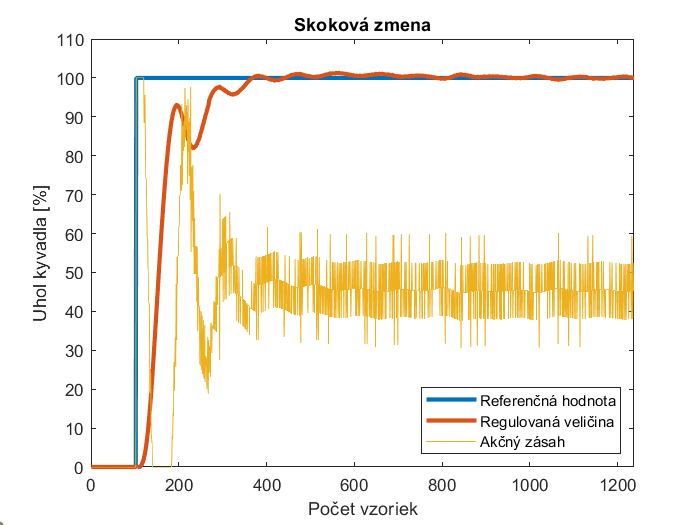
\includegraphics[width=120mm]{obr/SkokovaZmena.png}
	\caption{Reakcia systému na skokovú zmenu referenčnej hodnoty- Arduino IDE.}\label{OBRAZOK 2.5.1}
\end{figure}

Manuálna trajektória Obr. \ref{OBRAZOK 2.5.3}, má oproti automatickej trajektórii Obr. \ref{OBRAZOK 2.5.2}, väčšie rozdiely v hodnote akčného zásahu. Je to spôsobené kontinuálnou zmenou referenčnej hodnoty, ako aj miernym šumom signálu z potenciometra. V rámci Obr. \ref{OBRAZOK 2.5.3} si ešte môžeme všimnúť časť medzi vzorkami 5000-6000. Ide o manuálne zavedenie chyby, pomocou buchnutia do kyvadla. Systém na takúto zmenu reaguje zmenou akčného zásahu a regulačnú odchýlku menšiu ako 2\%, nadobúda v priebehu jednej sekundy. 

\begin{figure}[!tbh]
	\centering
	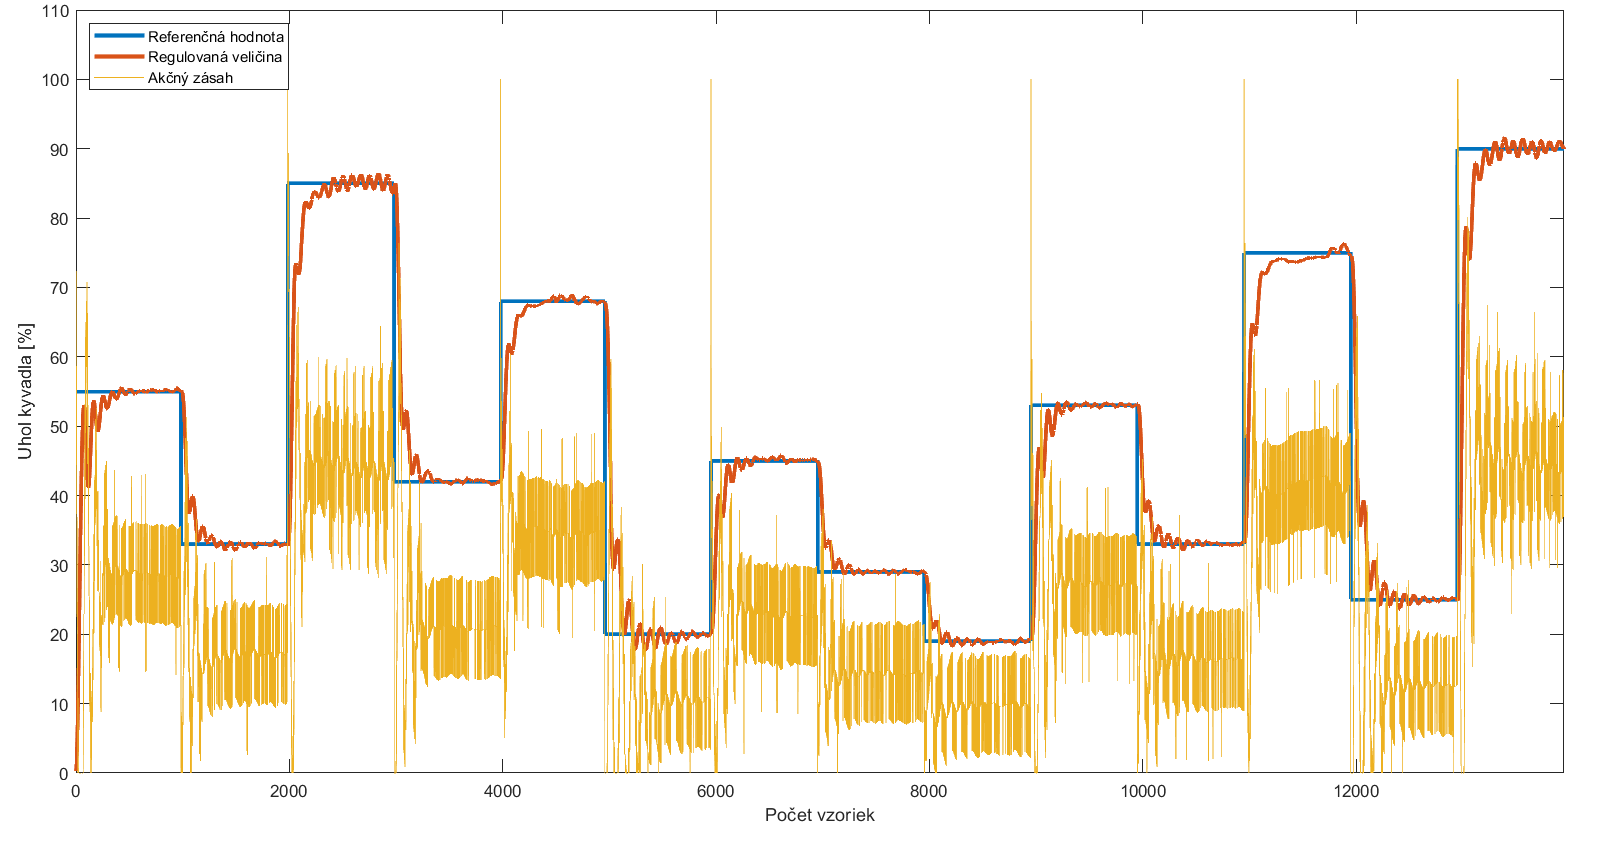
\includegraphics[width=150mm]{obr/Auto3.png}
	\caption{Automatická trajektória.}\label{OBRAZOK 2.5.2}
\end{figure}

\begin{figure}[!tbh]
	\centering
	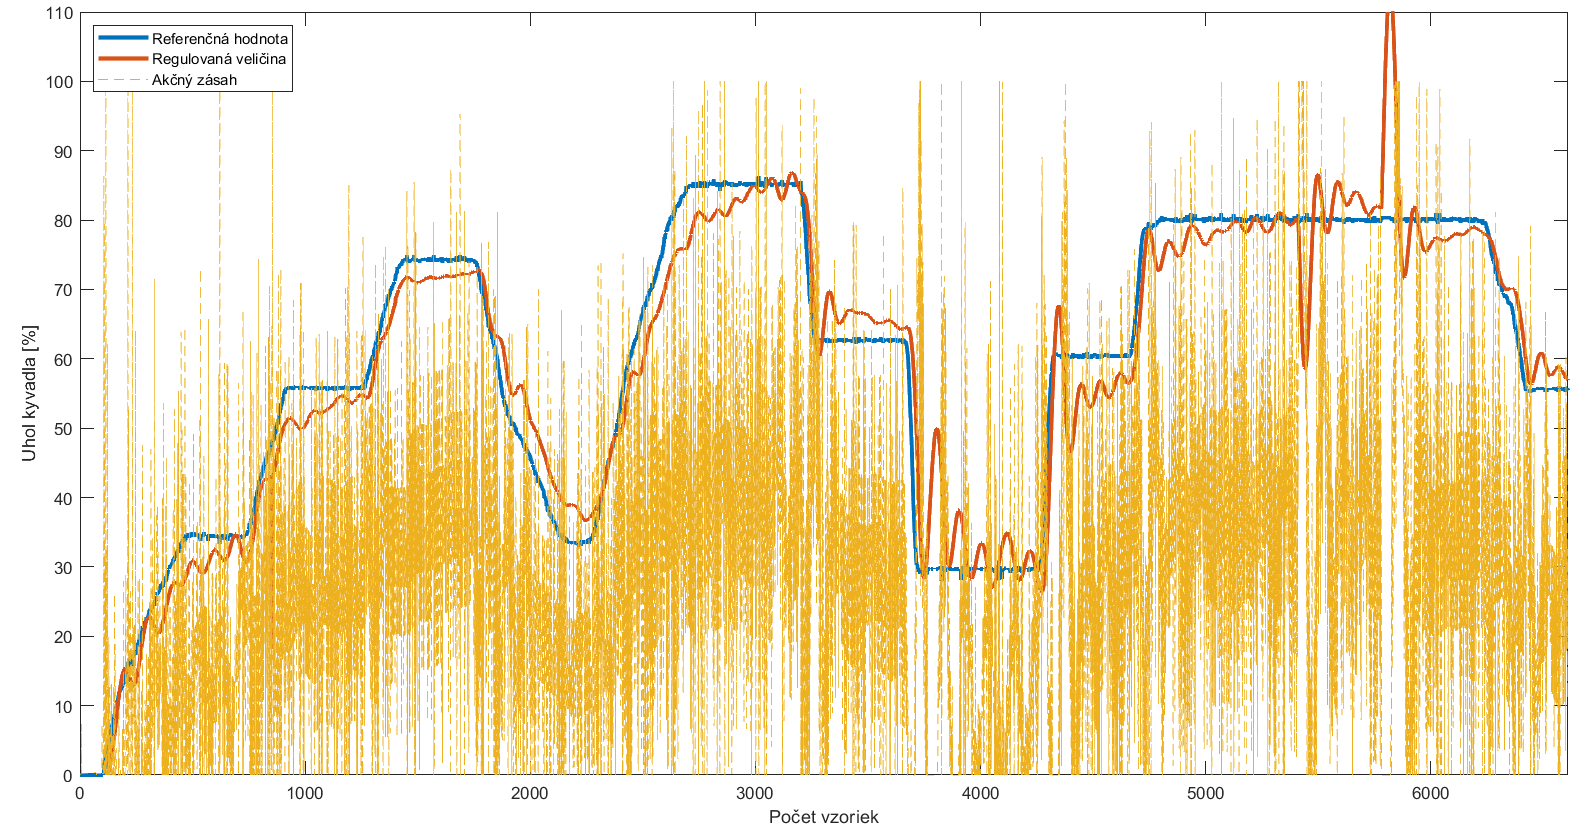
\includegraphics[width=150mm]{obr/potentio.png}
	\caption{Manuálna trajektória.}\label{OBRAZOK 2.5.3}
\end{figure}
